\documentclass[10pt,letterpaper]{article}

\usepackage{cogsci}
\usepackage{pslatex}
\usepackage{apacite}
\usepackage{amsmath}
\usepackage{graphicx}

\DeclareMathOperator*{\argmax}{arg\,max}

\title{Describing dynamics in classroom education using simple teaching games}
 
\author{{\large \bf Michael C. Frank} \\
  \texttt{mcfrank@stanford.edu} \\
  Department of Psychology\\
  Stanford University}


\begin{document}

\maketitle

\begin{abstract}
We describe a model of classroom teaching that construes teaching as communication to a heterogeneous audience. A number of basic educational results fall out of this construal, including (1) decreasing mean performance with the increasing size and variability among students in a class, (2) increases in performance based on grouping students by abilities, and (3) the value of formative evaluation to enhance teachers' knowledge of student ability.

\textbf{Keywords:} 
Bayesian modeling; agent-based modeling; education; pragmatics; teaching
\end{abstract}

\section{Introduction}

To fill this need, we describe a model of classroom teaching. This model captures phenomena that have to do with the informational dynamics of the classroom---how much information can be transferred between a teacher and a group of students with certain abilities and prior beliefs. It has nothing to say about another---perhaps ultimately more important---part of the classroom experience, its motivational dynamics.  

What are the functions of such a model? 

\section{Teaching games}

The basic unit of our analysis is a teaching game. In such a game, teacher $T$ attempts to provide information to students $S = {s_1 ... s_n}$. Teacher conveys information by choosing examples $E = {e_1 ... e_m}$ to illustrate an underlying concept $C$, based on some estimate of the students' prior knowledge and abilities $\hat{S} = {\hat{s_1} ... \hat{s_m}}$. Learners in turn attempt to recover $C$ with maximal fidelity. The teacher's payoff is determined by a test, administered to each of the learners. 

We will begin by considering a very simple form of this sort of game, with one example, perfect teacher knowledge of students, and perfect testing of student's knowledge. In this game, the concept to be learned is the distribution of a Bernoulli variable (the weight on a coin, e.g.). The teacher has some knowledge state, represented by a distribution over coin weights, which she wishes to impart to the students. She can make one choice, which is whether to show all of the students a coin flip showing heads or showing tails.

\subsection{Students}

\begin{figure}[t]
\begin{center}
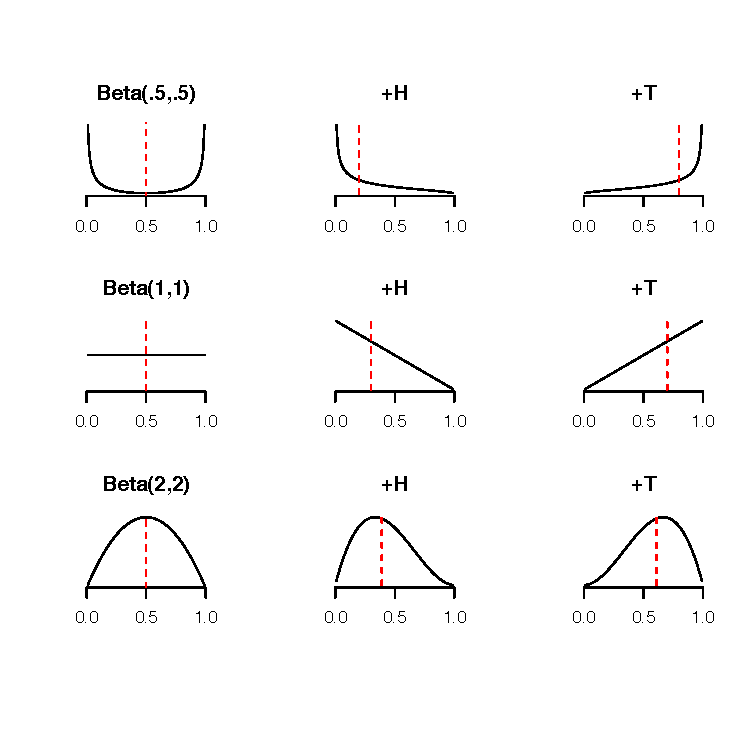
\includegraphics[width=3.5in]{figures/students.pdf}
\end{center}
\caption{\label{fig:students} Examples of the beta-bernoulli distribution with different priors and patterns of evidence. Black curves show probability distribution with a given prior (left column) and after observing a single tail or head (middle and right columns). Red lines show posterior mean.}
\end{figure}

We model the student here as a Bayesian (optimal) estimator of the target Bernoulli distribution, using a conjugate Beta-Bernoulli distribution. This model is very convenient: the form of the prior distribution is $Beta(\alpha,\beta)$, and the form of the posterior can be written $Beta(\alpha+t,\beta+h)$ where $t$ and $h$ represent the number of heads (0) and tails (t) observed in the data respectively. In this sense, if $t$ and $h$ are the \emph{counts} of observed data, then $\alpha$ and $\beta$ can be referred to as \emph{pseudo-counts}.

This formulation also gives us a way to model both the student's abilities and their prior knowledge about the situation. Consider the example Beta-Bernoulli distributions shown in Figure \ref{fig:students}. Symmetric priors of $\alpha=\beta=.5$ lead to a bias that the target coin weight is either 0 or 1, while $\alpha=\beta=.5$ leads to a bias towards fairer coins. As the strength of the prior grows, the effect of observing a single coin flip becomes weaker.

Under this formulation, the prior controls both the speed at which a student will learn and their overall bias. For example, as $\alpha$ and $\beta$ both go towards 0, the student's estimate converges to a maximum-likelihood estimate based on the observed data alone. In contrast, as $\alpha$ and $\beta$ both get larger, the student makes less and less use of the data and is more and more reliant on the shape of the prior distribution. The relative weights of $\alpha$ and $\beta$ control the student's bias---greater pseudo-counts on one or the other will lead to greater bias to believe that the correct parameter is lower or higher. We explore each of these scenarios---learning speed and bias---below.\footnote{For convenience below, we use a parameterization of the Beta distribution in terms of shape $\mu$ and scale $\nu$, where $\mu=\alpha / \alpha + \beta$ and $\nu = \alpha + \beta$. $\mu$ is equivalent to bias while $\nu$ captures speed.}

\subsection{Evaluation}

We are interested in computing the information gain caused by the teacher's particular example. For this purpose, we simulate perfect testing of students' knowledge both before and after the teacher shows her chosen example. We compute this via information theoretic measures. We notate the Beta distribution of the teacher's beliefs as $B_T$ = $Beta(\alpha_T,\beta_T)$, and similarly the student's Beta distributions before and after seeing the teacher's example as $B_{S}$ and $B_{S+e}$ respectively. This allows us to compute the Kullback-Leibler divergence \cite{cover2006} between student and teacher, both before and after seeing example $e$. The divergence between these two quantities is the information gain due to the example:

\begin{equation}
IG(e) = D_{KL} ( B_{S'})||B_T )  - D_{KL} ( B_{S+e} ||B_T ) 
\end{equation}

\noindent where the divergence measure is computed

\begin{equation}
\begin{split}
D_{KL} ( B_{S})||B_T )  = & \log( \frac{B(\alpha_{S},\beta_{S})}{B(\alpha_{T},\beta_{T})}) + \\
& (\alpha_T - \alpha_S) \psi (\alpha_T) + \\ 
& (\beta_T - \beta_S) \psi (\beta_T) + \\
& (\alpha_T - \alpha_S + \beta_T - \beta_S) \psi (\alpha_T + \beta_T).
\end{split}
\end{equation}

\subsection{Teachers}

Teachers are assumed to choose between possible examples in the set $E$ so as to maximize the average information gain across students. Thus their expected information gain is the information gain due to the best example that they could show:

\begin{equation}
E[IG] = \argmax_e {IG(e)}.
\end{equation}

Note that this formulation assumes that they have perfect knowledge of the students both before and after an example, and can mentally simulate the effects of a particular example on student knowledge, so as to pick the appropriate one. 

\section{Simulations}

We use this model 

\subsection{Classroom size}

\subsection{Tracking}

\subsection{Testing for better knowledge}

\section{Decision-theoretic analyses}


\section{Acknowledgments}

Thanks to Noah Goodman, Long Ouyang, and Roger Levy for valuable discussion.

\bibliographystyle{apacite}

\setlength{\bibleftmargin}{.125in}
\setlength{\bibindent}{-\bibleftmargin}

\bibliography{teaching}


\end{document}
